\chapter{Revisão da Literatura}
\citeonline{Moh06} desenvolveram um trabalho utilizando MD no qual o objetivo foi desenvolver modelos para classificação de doenças do arroz egípcio. Um dos algoritmos de aprendizagem utilizado foi a RNA. A RNA foi construída e treinada utilizando uma configuração de 52 entradas, 33 neurônios na camada oculta, 5 saídas, taxa de aprendizagem de 0.3, momento de 0.2 e 500 iterações. O modelo obtido para a previsão de doenças de arroz atingiu um índice de acerto de 96,4\% para o conjunto de dados de teste. Este resultado demonstra a grande eficiência da aplicação de RNAs.

\citeonline{Bla99} realizaram a comparação entre RNA e analise discriminante para criação de classificadores para tipos de coberturas florestais a partir de variáveis cartográficas. O RNA construída utilizou as configurações de 54 entradas, 120 neurônios na camada oculta, 7 classes de tipos de coberturas florestais, com uma taxa de aprendizagem de 0.05, taxa de momento de 0.5 e 1000 interações. Para obter estas configurações para a RNA foram realizados 56 analises diferentes demandando de cerca de 56 horas para cada analise. Após a comparação das técnicas, as RNAs obtiveram uma maior precisão, chegando a 70,58\%.

\citeonline{Ala05} observou que quando o processo de aprendizado de um modelo por meio de algoritmos de aprendizagem é iniciado, este com um grande conjunto de dados, ou com um alto número de repetições, demanda de um alto custo computacional e tempo de execução. Por meio destas observações, Guimarães desenvolveu um aplicativo para distribuir o processamento da construção de seu modelo, por meio do qual o processamento poderia ser realizado por vários computadores, utilizando o algoritmo de aprendizagem Algoritmos Genéticos (AG). Este aplicativo obteve bons resultados conseguindo reduzir seu tempo de execução estimado para construção do modelo de 1450 horas para 84 horas.

\citeonline{Sou11} aplicaram uma ferramenta de MD em paralelo para construção de um modelo de classificação utilizando RNA para produção de soja, afim de observar a relação existente entre os atributos químicos do solo e a produção. Utilizando apenas um computador eles reduziram o tempo de processamento de 280 para 80 segundos. Esses resultados demostraram que a utilização de técnicas de computação paralela podem melhorar significativamente o tempo de resposta das atividades de mineração.

O processo de mineração de dados é ilustrado na Figura~\ref{fig:mineracao}.
\begin{figure}
	\centering
	\caption{Etapas da mineração de dados}\label{fig:mineracao}
	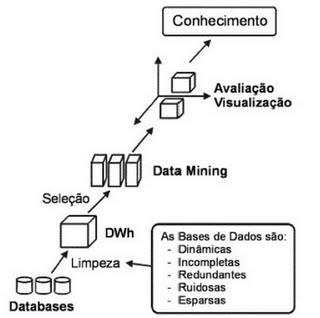
\includegraphics[scale=1.0]{mineracao}
	
\end{figure}


